\chapter{Estado del Arte}
\label{ch:estadoDelArte}

En el caso de las imágenes obtenidas por resonancia magnética, lo que se obtiene son un
arreglo de imágenes de distintos niveles en un mismo eje geométrico de un cuerpo. Luego, para
generar una malla geométrica del cuerpo existen diversas técnicas, muchas de ellas basadas en
\jcq{voxels} como por ejemplo, Marching Cubes\cite{Lorensen87marchingcubes}, Marching Tetrahedrons\cite{Shirley90apolygonal} y Marching Diamonds.
En esta investigación se dará especial énfasis en el algoritmo de Marching Cubes, se
explicará su funcionamiento, resultados y problemas que actualmente presenta.
Para entender mejor cómo funciona Marching Cubes, es de utilidad primero ver el caso
reducido a dos dimensiones, el que puede ser llamado como \jcq{Marching Squares}.

\section{Marching Squares}
\label{sec:marchingSquares}

En dos dimensiones, para obtener el contorno de una figura, se puede usar este algoritmo
que se basa en crear divisiones cuadradas uniformes del espacio, y en cada una de ellas dibujar un
patrón específico del caso que encierra esa división, finalmente todas las divisiones tienen
dibujadas un patrón específico o un espacio vacío, obteniendo así el contorno de la imagen
tratada. El siguiente caso, ejemplifica el proceso completo.

Se supone la imagen de la figura \ref{f:estadoDelArte:original} para tratar obtener su contorno.

\begin{figure}
	\centering
		\fbox{
			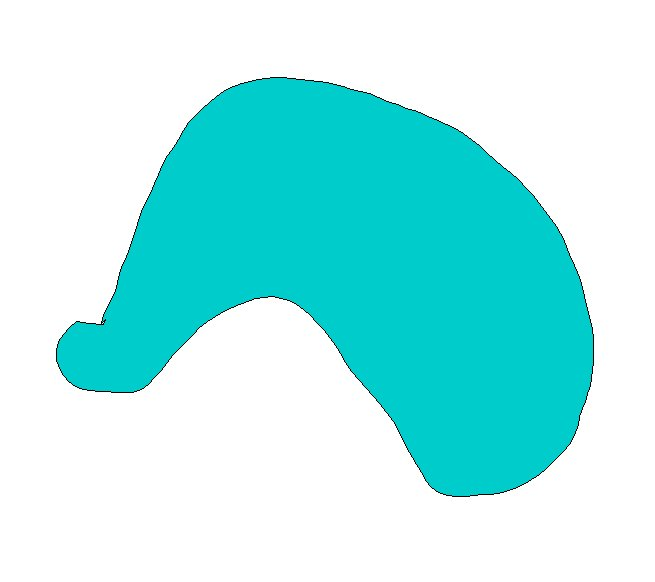
\includegraphics[width=0.7\textwidth]{images/marchingsquare/original.jpg}
		}
	\caption{Figura original de estudio, a la que se desea extraer su contorno}
	\label{f:estadoDelArte:original}
\end{figure}

Luego se divide el espacio en un arreglo uniforme de cuadriláteros, en este caso una
matriz de 7x8 celdas como muestra la figura \ref{f:estadoDelArte:division}

Para poder obtener el patrón a dibujar en cada celda, se hace un proceso de
reconocimiento. En un principio es necesario etiquetar cada vértice de cada celda dependiendo si
están dentro o fuera de la región de interés. Esto puede ser calculado de distintas formas que
dependen intrínsecamente del problema, para este caso, basta con detectar si el vértice está sobre
un pixel blanco o no, en otros casos, puede depender de que si el valor del pixel en escala de
grises supera (o es inferior) a un valor fijo determinado por el científico.

\begin{figure}
	\centering
		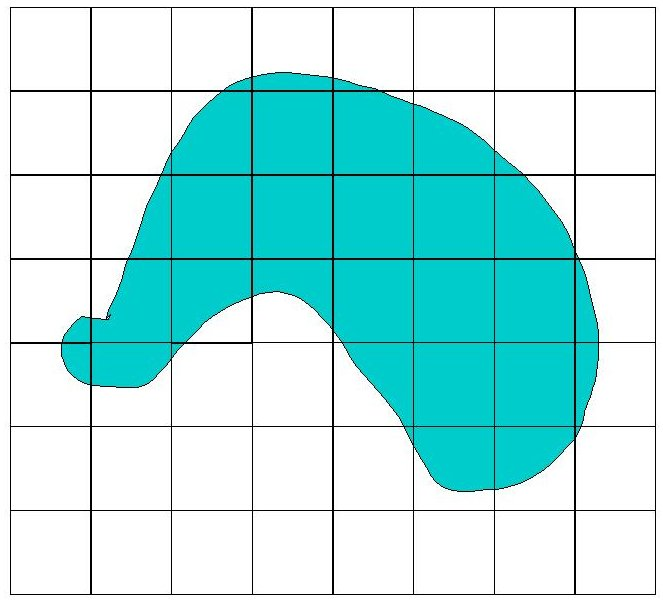
\includegraphics[width=0.7\textwidth]{images/marchingsquare/division.jpg}
	\caption{Figura original dividida en un arreglo uniforme de celdas}
	\label{f:estadoDelArte:division}
\end{figure}

A continuación, se muestra como quedan etiquetados los vértices, dependiendo si están
dentro de la figura (en rojo), o si están fuera de la figura (en azul), como muestra la figura \ref{f:estadoDelArte:labeledobj}

\begin{figure}
	\centering
		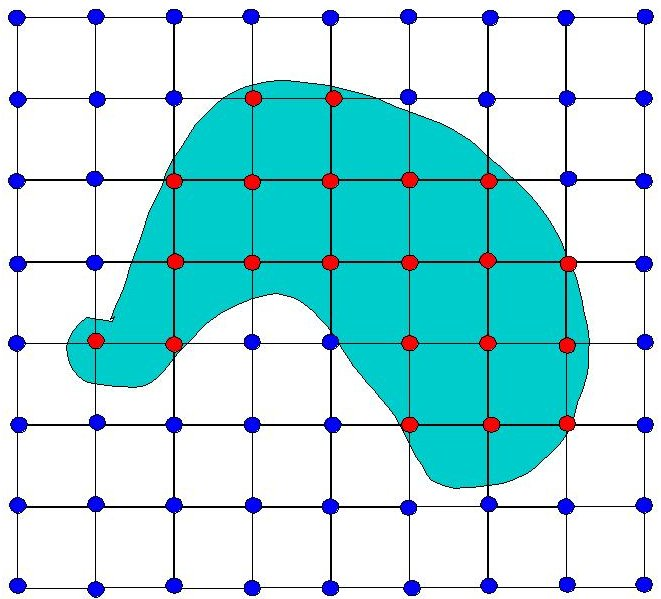
\includegraphics[width=0.7\textwidth]{images/marchingsquare/labeledobj.jpg}
	\caption{Etiquetado de vértices según su condición relativa a la figura}
	\label{f:estadoDelArte:labeledobj}
\end{figure}

Si ahora se analiza celda a celda, se ve que existen dieciséis combinaciones distintas de
vértices etiquetados como dentro o fuera de la región en una misma celda, como muestra la figura
\ref{f:estadoDelArte:cases}

\begin{figure}
\centering
	\fbox{
		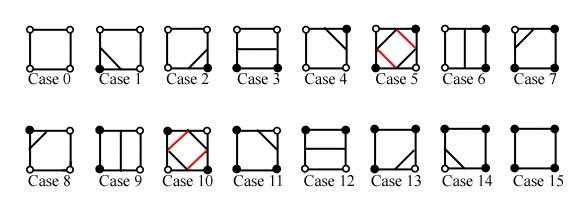
\includegraphics[width=\textwidth]{images/marchingsquare/cases.jpg}
	}
\caption{Los dieciséis casos posibles en Marching Squares}
\label{f:estadoDelArte:cases}
\end{figure}

Además se entiende que si uno de los lados de una celda (una arista) esta formada por un
vértice marcado como dentro y otro fuera, significa que por esa arista corta el borde de la figura,
y por lo tanto, esa arista la dejamos marcada como una arista de contorno detectada, que en este
ejemplo se marca de color morado, como muestra la figura \ref{f:estadoDelArte:purpledobj}

\begin{figure}
\centering
	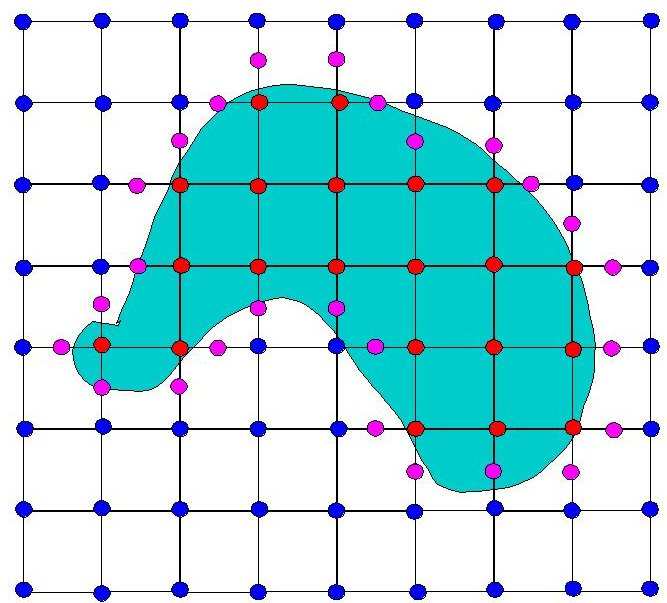
\includegraphics[width=0.7\textwidth]{images/marchingsquare/purpledobj.jpg}
\caption{Aristas marcadas por las cuales cortará el contorno calculado}
\label{f:estadoDelArte:purpledobj}
\end{figure}

Luego, por cada celda, se unen los puntos morados formados en el paso anterior, creando
así uno de los dieciséis patrones posibles, lo cual se puede entender como una de las dieciséis
formas en que un cuadrilátero puede ser atravesado por una linea, formando así el contorno
buscado, como muestra la figura \ref{f:estadoDelArte:connectedobj}

\begin{figure}
\centering
	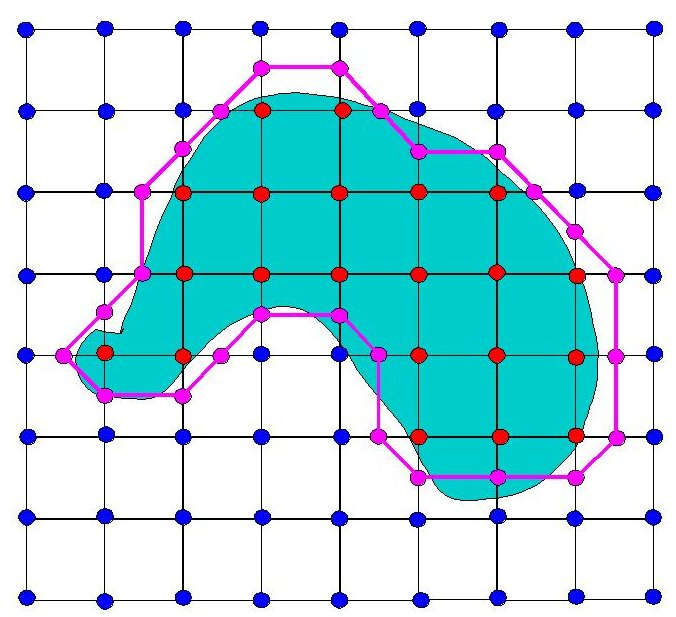
\includegraphics[width=0.7\textwidth]{images/marchingsquare/connectedobj.jpg}
\caption{Contorno calculado usando las aristas marcadas en el paso anterior}
\label{f:estadoDelArte:connectedobj}
\end{figure}

Posteriormente, dependiendo de los requerimientos de la investigación, se puede mejorar
la aproximación haciendo una interpolación lineal de los valores de los vértices para calcular en
que punto aproximadamente la figura (a la que se quiere extraer su contorno), corta con la arista,
un ejemplo del resultado de esta aproximación se muestra en la figura \ref{f:estadoDelArte:2Dintersected}

\begin{figure}
\centering
	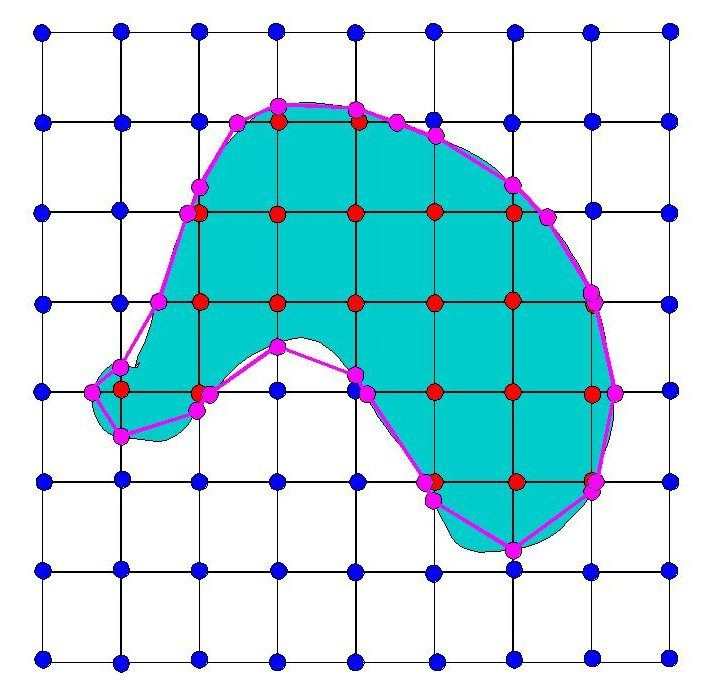
\includegraphics[width=0.7\textwidth]{images/marchingsquare/2Dintersected.jpg}
\caption{Mejorando la calidad del contorno usando interpolación lineal}
\label{f:estadoDelArte:2Dintersected}
\end{figure}

\subsection{Consecuencias}
\label{subsec:marchingSquares:consecuencias}

Evidentemente, existen ciertas falencias, por ejemplo, el contorno obtenido no simula
adecuadamente el objeto estudiado, debido a errores causados por la fragmentación de las
divisiones iniciales, una solución directa para mejorar esto es aumentar las divisiones, es decir,
hacer que todas las celdas sean mas pequeñas, y así hacer una mejor aproximación del contorno
del objeto en estudio. De la misma manera, existen otras técnicas, tales como hacer particiones
con celdas de tamaño variable en las particiones, o subdividir aquellas celdas que hayan sido
detectadas como de frontera y así obtener un mejor desempeño en el algoritmo.

Otro problema es que algunos casos presentan ambigüedad, es decir, no es trivial calcular
a cual caso pertenece una cierta configuración, por ejemplo, tomando el quinto y décimo caso
descritos anteriormente, se supone el ejemplo descrito por la figura \ref{f:estadoDelArte:marchingSAmbEx}

\begin{figure}[hbp]
\centering
	\fbox{
		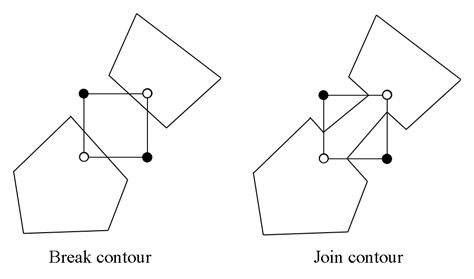
\includegraphics[width=0.7\textwidth]{images/marchingsquare/marchingSAmbEx.jpg}
	}
\caption{Casos con ambigüedad}
\label{f:estadoDelArte:marchingSAmbEx}
\end{figure}

Este cuadrado, tiene dos vértices diagonalmente opuestos marcados. Sin conocer como es
la figura ni cómo son las divisiones vecinas, no se puede saber con exactitud si se trata del quinto
o el décimo caso, por lo que el algoritmo puede erróneamente separar el contorno, formando así
dos figuras separadas, o las une, de manera que sólo exista una figura con un contorno
compartido.

\section{Marching Cubes}
\label{sec:marchingCubes}

\subsection{Idea}
\label{subsec:marchingCubes:idea}

Marching Cubes es un algoritmo de extracción de una superficie poligonal de un cuerpo
en un espacio escalar en tres dimensiones \cite{Lorensen87marchingcubes}. Existen muchas aplicaciones para este tipo de técnicas,
dos de las más comunes son:

\begin{itemize}
	\item Reconstrucción de una superficie a partir de un set de imágenes médicas, como
	por ejemplo los obtenidos en imágenes de resonancia magnética, los que pueden formar
	un volumen en tres dimensiones.

	\item Crear un contorno tridimensional de un campo escalar matemático, en este caso,
	el valor de una cierta función es conocido en todo el espacio, pero es representada como
	vértices de una malla tridimensional.
\end{itemize}

Adopta la misma idea que hay detrás de Marching Squares, pero llevando los conceptos a
tres dimensiones, en este caso, el dominio es un espacio tridimensional, en el cual existe un
cuerpo al que se desea extraer su superficie. Luego, el espacio es dividido en regiones uniformes
(cubos), por los cuales la superficie del objeto corta las aristas de estos cubos.

\subsection{Consideraciones Geométricas}
\label{subsec:marchingCubes:consideracionesGeometricas}

Un cubo tiene seis caras, ocho vértices y doce aristas, las cuales, para efectos de esta
investigación serán numeradas como se muestra en la figura \ref{f:estadoDelArte:convention}

%convencion FINAL
%TODO: al parecer quiza sea necesario usar una convencion equitativa, pero rotada
%para que considere los dataset como son interpretados, es decir, con Y positivo
%apuntando hacia abajo, y Z en direccion a donde se van poniendo las imagenes
%		3	2
%	0	1
%		7	6
%	4	5
\begin{figure}[hbp]
\centering
	\fbox{
		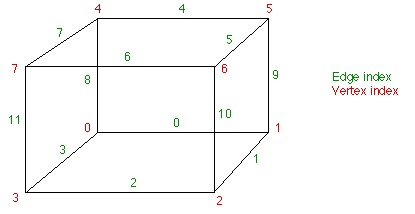
\includegraphics[width=0.9\textwidth]{images/marchingcubes/convention.jpg}
	}
\caption{Convención de enumeración de vértices y aristas}
\label{f:estadoDelArte:convention}
\end{figure}

De la misma manera que el caso de dos dimensiones, debido a que cada uno de los ocho
vértices puede tener dos estados: vértice marcado como interno o externo (dentro o fuera de la
superficie del cuerpo), se tienen 256 combinaciones posibles, es decir, una superficie puede
atravesar a un cubo de 256 maneras posibles. Sin embargo, al igual que en su homólogo en dos
dimensiones, que tiene dieciséis formas posibles, estas pueden ser reducidas a un número inferior
de patrones, ya que entre ellos existen diferencias solamente de rotación y reflexión.

En el caso de tres dimensiones, los 256 patrones pueden ser reducidos de la misma
manera. Dos de esos casos son triviales, ya que tienen todos sus vértices marcados como internos
o externos, por lo tanto, ambos casos no contribuyen a la superficie que se quiere extraer.

Si se consideran las simetrías, hay solamente catorce posibles configuraciones únicas en
los restantes 254 casos. Por ejemplo, aquellos casos que solamente tienen un vértice marcado
como interno, sólo representan un triángulo que atraviesa las aristas que convergen a ése vértice y
existen ocho casos como éste, uno por cada vértice del cubo.

Finalmente las quince familias de posibles casos son los que se describen en la figura \ref{f:estadoDelArte:Shu95adaptivemarching_1}

\begin{figure}[hbp]
\centering
	\fbox{
		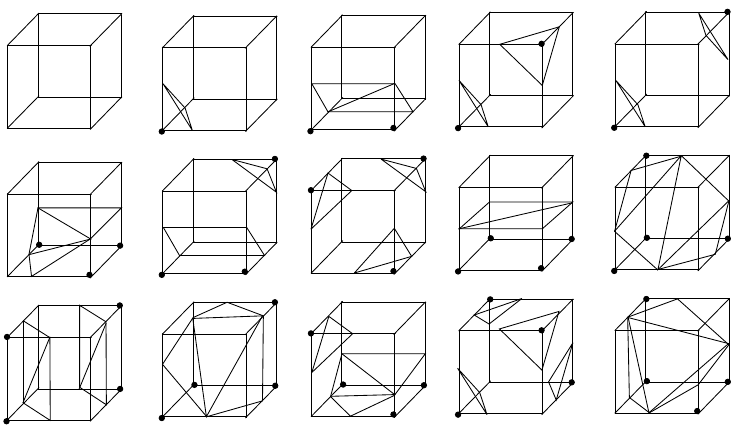
\includegraphics[width=0.9\textwidth]{images/marchingcubes/Shu95adaptivemarching_1.png}
	}
\caption{Los quince casos de Marching Cubes \cite{Shu95adaptivemarching}}
\label{f:estadoDelArte:Shu95adaptivemarching_1}
\end{figure}

\subsection{Procedimiento}
\label{subsec:marchingCubes:procedimiento}

El procedimiento es similar al explicado a Marching Squares, en primer lugar se divide el
espacio en un arreglo uniforme de regiones cúbicas, luego, se evalúa cada vértice para etiquetarlo como un vértice interno o externo, luego, calcular a cuál de los 15 casos pertenece cada división y generar los triángulos, para finalmente extraer así la superficie.
En resumen, el procedimiento reducido a un solo cubo, ocurre según lo siguiente:

En un comienzo se tiene un cubo, como el descrito en la figura \ref{f:estadoDelArte:cube_01}

\begin{figure}[hbp]
\centering
	\fbox{
		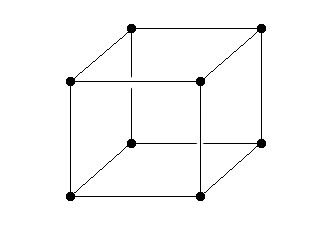
\includegraphics[width=0.4\textwidth]{images/marchingcubes/cube_01.png}
	}
\caption{Un cubo con sus vértices marcados}
\label{f:estadoDelArte:cube_01}
\end{figure}

Suponiendo que este cubo tiene solamente un vértice que quedó dentro del cuerpo, éste
vértice queda marcado como un vértice interno (en rojo), los siete restantes quedan marcados
como vértices externos (en negro), descrito por le figura \ref{f:estadoDelArte:cube_02}

\begin{figure}[hbp]
\centering
	\fbox{
		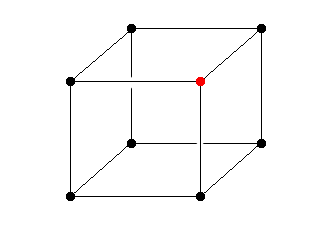
\includegraphics[width=0.4\textwidth]{images/marchingcubes/cube_02.png}
	}
\caption{Un cubo con uno de sus vértices marcado como interno}
\label{f:estadoDelArte:cube_02}
\end{figure}

Luego se crea un triángulo cuyos vértices se apoyan en los puntos medios de las aristas
que comparten el vértice marcado como interno, de esta manera, se tiene un cubo que es
atravesado por una superficie que precisamente deja un solo vértice dentro (o fuera, dependiendo
de la reflexión del caso), resultando un triángulo como el de la figura \ref{f:estadoDelArte:cube_03}

\begin{figure}[ht]
\centering
	\fbox{
		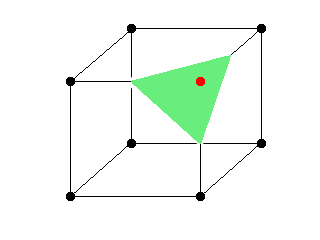
\includegraphics[width=0.4\textwidth]{images/marchingcubes/cube_03.png}
	}
\caption{Un triángulo atraviesa el cubo separando el vértice marcado de los demás}
\label{f:estadoDelArte:cube_03}
\end{figure}

\subsection{Consecuencias}
\label{subsec:marchingCubes:consecuencias}

Nuevamente, al igual que su versión en dos dimensiones, presenta las mismas falencias.
Por ejemplo, sin ninguna interpolación y dependiendo de la resolución de la división, la
superficie extraída puede presentar un efecto de escalonamiento (\jcq{aliasing}) como se
muestra en la figura \ref{f:estadoDelArte:superficies_resultantes_variando_divisiones}

\begin{figure}

	\begin{subfigure}{0.45\textwidth}
		\centering
		\includegraphics[width=\textwidth]{images/marchingcubes/mc_blobs.png}
		\caption{La forma original}
		\label{f:estadoDelArte:mc_blobs}
	\end{subfigure}
	~
	\begin{subfigure}{0.45\textwidth}
		\centering
		\includegraphics[width=\textwidth]{images/marchingcubes/mc_blobs_12.png}
		\caption{Marching Cubes con 12 divisiones}
		\label{f:estadoDelArte:mc_blobs_12}
	\end{subfigure}

	\begin{subfigure}{0.45\textwidth}
		\centering
		\includegraphics[width=\textwidth]{images/marchingcubes/mc_blobs_20.png}
		\caption{Marching Cubes con 20 divisiones}
		\label{f:estadoDelArte:mc_blobs_20}
	\end{subfigure}
	~
	\begin{subfigure}{0.45\textwidth}
		\centering
		\includegraphics[width=\textwidth]{images/marchingcubes/mc_blobs_50.png}
		\caption{Marching Cubes con 50 divisiones}
		\label{f:estadoDelArte:mc_blobs_50}
	\end{subfigure}

	\caption{Superficies resultantes variando la cantidad de divisiones}
	\label{f:estadoDelArte:superficies_resultantes_variando_divisiones}
\end{figure}

Se puede apreciar que al aumentar la resolución, la calidad aumenta, pero
computacionalmente requiere mas cómputo y memoria ya que aumenta la cantidad de caras que
describen la superficie extraída como se ve en la figura \ref{f:estadoDelArte:polygonise3}

\begin{figure}[!ht]
\centering
	\fbox{
		\includegraphics[width=0.9\textwidth]{images/marchingcubes/polygonise3.png}
	}
\caption{Ejemplificación de cómo varían los resultados al modificar la resolución}
\label{f:estadoDelArte:polygonise3}
\end{figure}

El principal problema de \emph{Marching Cubes} es que existe la posibilidad de que aparezcan agujeros como el resultado de la discrepancia en la conexión de los vértices en una cara en común de dos cubos adyacentes \cite{Chernyaev95marchingcubes}

Como se muestra en la figura \ref{f:estadoDelArte:Bloomenthal88polygonizationof_1}, la poligonización puede producir casos ambigüos cuando en una cara de un cubo quedan marcados dos vértices opuestos (que no comparten ninguna arista), ya que no es posible decidir si la superficie corta en multiples partes el cubo o un cilindro atraviesa las dos esquinas opuestas.

\begin{figure}[t]
\centering
	\fbox{
		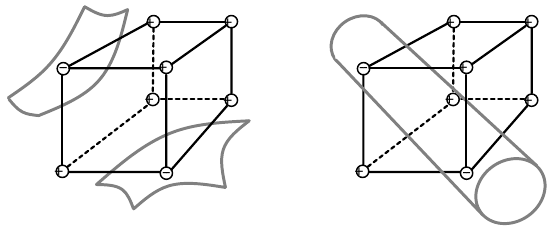
\includegraphics[width=0.7\textwidth]{images/marchingcubes/Bloomenthal88polygonizationof_1.png}
	}
\caption{Casos en los que se generan errores topológicos}
\label{f:estadoDelArte:Bloomenthal88polygonizationof_1}
\end{figure}

Es por esto que si se forma una configuración en la que dos cubos comparten una cara las cuales tienen solo dos vértices opuestos marcados, pueden generar agujeros en el modelo final en tres dimensiones, como se grafica en la figura \ref{f:estadoDelArte:Chernyaev95marchingcubes_1}

\begin{figure}[!htb]
\centering
	\fbox{
		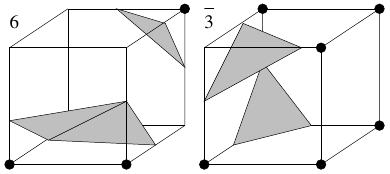
\includegraphics[width=0.5\textwidth]{images/marchingcubes/Chernyaev95marchingcubes_1.png}
	}
\caption{Un agujero causado por una cara con ambigüedad compartida por dos cubos \cite{Chernyaev95marchingcubes}}
\label{f:estadoDelArte:Chernyaev95marchingcubes_1}
\end{figure}

Otro problema puede incluso aparecer cuando no hay discrepancias visibles, \emph{Marching Cubes} puede producir \emph{isosuperficies} con una topología diferente a la generada por otros métodos en el mismo caso \cite{Chernyaev95marchingcubes}. La figura \ref{f:estadoDelArte:Chernyaev95marchingcubes_2} muestra las \emph{isosuperficies} generadas para el mismo cubo usando dos metodos distintos, el primer método se realizó usando \emph{Marching Cubes} y el otro usando \emph{Dividing Cubes Method} \cite{Cline88twoalgorithms}, el cual subdivide el cubo en regiones cúbicas mas pequeñas. La superficie generada por \emph{Marching Cubes} consiste en dos triángulos separados, mientras que la superficie generada por \emph{Dividing Cubes Method} parece mas un \jcq{tubo}

\begin{figure}[tb]
\centering
	\fbox{
		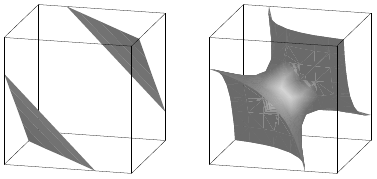
\includegraphics[width=0.5\textwidth]{images/marchingcubes/Chernyaev95marchingcubes_2.png}
	}
\caption{\emph{isosuperficies} generadas por dos métodos diferentes \cite{Chernyaev95marchingcubes}}
\label{f:estadoDelArte:Chernyaev95marchingcubes_2}
\end{figure}

Resolviendo las ambigüedades, se pueden evitar los agujeros, de todas maneras, esto no garantiza una topología correcta \cite{Lewiner03efficientimplementation}, tambien es necesario resolver las ambigüedades internas, causadas por aquellos casos que tienen vértices marcados y diagonalmente opuestos. Por ejemplo, para un mismo caso, pueden existir dos posibles poligonizaciones que resuelven el caso y son topológicamente distintas como se muestra en la figura \ref{f:estadoDelArte:Lewiner03efficientimplementation_2}

\begin{figure}[!htb]
\centering
	\fbox{
		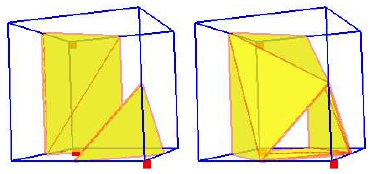
\includegraphics[width=0.5\textwidth]{images/marchingcubes/Lewiner03efficientimplementation_2.png}
	}
\caption{Dos posibles poligonizaciones para el mismo caso, ambas resuelven los dos posibles casos de ambigüedad \cite{Lewiner03efficientimplementation}}
\label{f:estadoDelArte:Lewiner03efficientimplementation_2}
\end{figure}

Estos problemas pueden ser eliminados si se usa una particion del espacio usando \emph{simplexs}.
Un \emph{simplex} es la descomposición lineal más simple de un n-espacio. Para tres dimensiones, es el tetraedro \cite{Bloomenthal88polygonizationof}. Cualquier par de vértices de un tetraedro esta unido por una arista en común, y por lo tanto, cualquier vértice marcado puede ser separado del resto usando solamente un plano.

Actualmente existen implementaciones que usan tetraedros en lugar de cubos para la poligonización con el fin de evitar este problema de la ambigüedad, y se basan en dividir el cubo en tetraedros, dependiendo la implementación, el cubo puede ser dividido en cinco \cite{BAPayne90surfacemapping}, seis, e incluso doce \cite{Bloomenthal88polygonizationof} tetraedros, como se muestra en la figura \ref{f:estadoDelArte:divisionesTetraedricasDeUnCubo}

\begin{figure}[h]

	\begin{subfigure}[b]{0.45\textwidth}
		\centering
		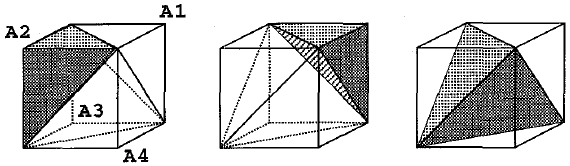
\includegraphics[width=\textwidth]{images/marchingcubes/GueziecHummel95exploitingtriangulated_1.png}
		\caption{Cinco divisiones tetraédricas}
		\label{f:estadoDelArte:cincoDivisionesTetraedricas}
	\end{subfigure}
	~
	\begin{subfigure}[b]{0.45\textwidth}
		\centering
		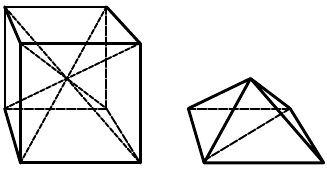
\includegraphics[width=\textwidth]{images/marchingcubes/Bloomenthal88polygonizationof_2.png}
		\caption{Doce divisiones tetraédricas}
		\label{f:estadoDelArte:doceDivisionesTetraedricas}
	\end{subfigure}

	\caption{Divisiones tetraédricas de un cubo}
	\label{f:estadoDelArte:divisionesTetraedricasDeUnCubo}
\end{figure}

Las principales diferencias de cada forma de dividir un cubo en una cierta cantidad de tetraedros, es que al tener menos tetraedros, se generan menos triángulos y viceversa, el problema de usar cinco tetraedros es que es necesario crear una division tetraedrica en forma de \jcq{espejo}, ya que los vértices de un tetraedro no coinciden con el tetraedro del siguiente cubo, por lo que hay que alternar estas dos particiones tetraedricas a modo de \jcq{tablero de ajedrez}, esto se puede evitar haciendo una particion distinta que sea consistente con los cubos vecinos, pero esto implica usar una particion con una cantidad mayor de tetraedros para asegurar esta caracteristica, lo que en la superficie final supone más triángulos. En cualquier caso, los problemas de ambigüedad de \emph{Marching Cubes} se eliminan usando divisiones tetraédricas.